\chapter{Test 01 Corrections}

\begin{prob} 10pts
\begin{subprob}
Correct
\end{subprob}
\begin{subprob}
Correct
\end{subprob}
\end{prob}
\begin{prob}
$A=
\begin{bmatrix}
   1 & 2 & 1\\
   -3 & -1 & 2\\
   0 & 5 & 3\\
\end{bmatrix}$ and $B=\begin{bmatrix}
   0 \\
   5 \\
   -1 \\
\end{bmatrix}$\\
\begin{align*}
&\begin{bmatrix}
   1 & 2 & 1 & | & 0\\
   -3 & -1 & 2 & | & 5\\
   0 & 5 & 3 & | & -1\\
\end{bmatrix}\\
r_2\rightarrow r_2+3r_1&\begin{bmatrix}
   1 & 2 & 1 & | & 0\\
   0 & 5 & 5 & | & 5\\
   0 & 5 & 3 & | & -1\\
\end{bmatrix}\\
r_2\rightarrow r_2/5&\begin{bmatrix}
   1 & 2 & 1 & | & 0\\
   0 & 1 & 1 & | & 1\\
   0 & 5 & 3 & | & -1\\
\end{bmatrix}\\
r_3\rightarrow r_3-5r_2&\begin{bmatrix}
   1 & 2 & 1 & | & 0\\
   0 & 1 & 1 & | & 1\\
   0 & 0 & -2 & | & -6\\
\end{bmatrix}\\
r_3\rightarrow r_3/-2&\begin{bmatrix}
   1 & 2 & 1 & | & 0\\
   0 & 1 & 1 & | & 1\\
   0 & 0 & 1 & | & 3\\
\end{bmatrix}\\
r_1\rightarrow r_1-2r_2&\begin{bmatrix}
   1 & 0 & -1 & | & -2\\
   0 & 1 & 1 & | & 1\\
   0 & 0 & 1 & | & 3\\
\end{bmatrix}\\
r_1\rightarrow r_1+r_3&\begin{bmatrix}
   1 & 0 & 0 & | & 1\\
   0 & 1 & 1 & | & 1\\
   0 & 0 & 1 & | & 3\\
\end{bmatrix}\\
r_2\rightarrow r_2-r_3&\begin{bmatrix}
   1 & 0 & 0 & | & 1\\
   0 & 1 & 0 & | & -2\\
   0 & 0 & 1 & | & 3\\
\end{bmatrix}\\
\end{align*}
Yes, B is in the subset spanned by the columns of A.
$$0\begin{bmatrix}
   1 \\
   -3 \\
   0 \\
\end{bmatrix}+5\begin{bmatrix}
   2 \\
   -1 \\
   5 \\
\end{bmatrix}-1\begin{bmatrix}
   1 \\
   2 \\
   3 \\
\end{bmatrix}=\begin{bmatrix}
   1 \\
   -2 \\
   3 \\
\end{bmatrix}$$
\end{prob}
\begin{prob}
Yes, the figure does have a solution; if you express the vectors as a linear combination $x_1v_1+x_2v_2+x_3v_3=b$ you can change the values of the scalars ($x_1$, $x_2$, $x_3$) to any value which, when multiplied by the vectors will give us any b; which causes the answer to b to be non-unique.

\begin{center}
    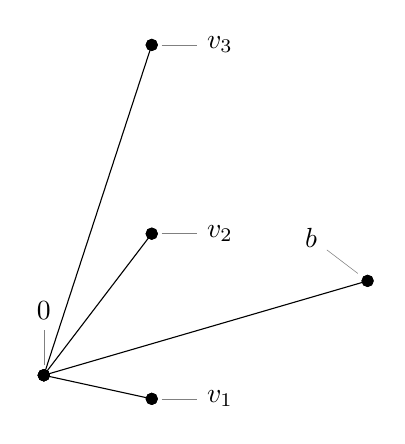
\begin{tikzpicture}
\begin{axis}[
    hide axis,
    xmin=-1, xmax=4,
    ymin=-1.5, ymax=8,
]
 
 \addplot[mark=*] coordinates {(0,0)} node[pin=90:{$0$}]{};
  \addplot[mark=*] coordinates {(1,7)} node[pin=0:{$v_3$}]{};
   \addplot[mark=*] coordinates {(3,2)} node[pin=150:{$b$}]{};
      \addplot[mark=*] coordinates {(1,-.5)} node[pin=0:{$v_1$}]{};
         \addplot[mark=*] coordinates {(1,3)} node[pin=0:{$v_2$}]{};
\addplot[mark=oplus] coordinates {(0,0)(1,7) };
    \addplot[mark=oplus] coordinates {(0,0)(1,3)};
    \addplot[mark=oplus] coordinates {(0,0)(3,2)};
 \addplot[mark=oplus] coordinates {(0,0)(1,-.5)};
\end{axis}
\end{tikzpicture}
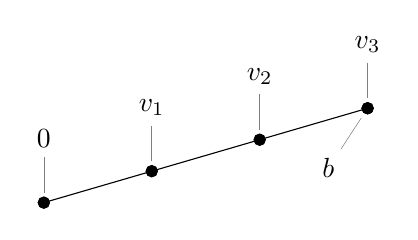
\begin{tikzpicture}
\begin{axis}[
    hide axis,
    xmin=-1, xmax=4,
    ymin=-1.5, ymax=8,
]
 
 \addplot[mark=*] coordinates {(0,0)} node[pin=90:{$0$}]{};
  \addplot[mark=*] coordinates {(3,2)} node[pin=90:{$v_3$}]{};
   \addplot[mark=*] coordinates {(3,2)} node[pin=240:{$b$}]{};
      \addplot[mark=*] coordinates {(1,2/3)} node[pin=90:{$v_1$}]{};
         \addplot[mark=*] coordinates {(2,4/3)} node[pin=90:{$v_2$}]{};
\addplot[mark=*] coordinates {(0,0)(1,2/3)(2,4/3)(3,2) };
\end{axis}
\end{tikzpicture}
\end{center}
\end{prob}
\begin{prob} 10pts
\begin{subprob}
\begin{align*}
&\begin{bmatrix}
   1 & 3 & 1\\
   0 & 3 & 6\\
   0 & 0 & 0\\
\end{bmatrix}\\
r_1\rightarrow r_1-r_2&\begin{bmatrix}
   1 & 0 & -5\\
   0 & 3 & 6\\
   0 & 0 & 0\\
\end{bmatrix}\\
r_2\rightarrow r_2/3&\begin{bmatrix}
   1 & 0 & -5\\
   0 & 1 & 2\\
   0 & 0 & 0\\
\end{bmatrix}\\
1x_1-5x_3&=0\\
1x_2+2x_3&=0\\
x_1&=5x_3\\
x_2&=-2x_3\\
x_3&=x_3\\
\begin{bmatrix}
   x_1\\
   x_2\\
   x_3\\
\end{bmatrix}&=\begin{bmatrix}
   5x_3\\
   -2x_3\\
   0\\
\end{bmatrix}\\
\begin{bmatrix}
   5x_3\\
   -2x_3\\
   0\\
\end{bmatrix}&=x_3\begin{bmatrix}
   5\\
   -2\\
   0\\
\end{bmatrix}
\end{align*}
\end{subprob}
\begin{subprob}
$$0\begin{bmatrix}
   5\\
   -2\\
   0\\
\end{bmatrix} = \begin{bmatrix}
   0\\
   0\\
   0\\
\end{bmatrix}$$
\end{subprob}
\begin{subprob}
Yes, $x_3$ is a free variable, any value will have a solution.
\end{subprob}
\end{prob}
\begin{prob} 30pts
\begin{subprob}
Correct
\end{subprob}
\begin{subprob}
Yes, because there is no way to reduce the matrices to be in the other matrix.
\end{subprob}
\begin{subprob}
No, it is linearly dependent because $v_1$, $v_2$ are dependant.
\end{subprob}
\begin{subprob}
No, because the vectors are not necessarily related.
\end{subprob}
\begin{subprob}
Yes, because the columns are related and a part of the same system.
\end{subprob}
\begin{subprob}
Yes, there are pivots in each column and there is no free variable therefore the sets are independant of each other.
\end{subprob}
\end{prob}
\begin{prob}
$\begin{bmatrix}
   2\\
   0\\
\end{bmatrix}-3\begin{bmatrix}
   3\\
   2\\
\end{bmatrix}=\begin{bmatrix}
   2\\
   0\\
\end{bmatrix}-\begin{bmatrix}
   9\\
   6\\
\end{bmatrix}=\begin{bmatrix}
   -7\\
   -6\\
\end{bmatrix}$
\end{prob}
\begin{prob} 10pts
\begin{center}
    \begin{tikzpicture}
\begin{axis}[
axis lines = center,
    xmin=-5, xmax=5,
    ymin=-5, ymax=5,
]
 
\addplot [
    domain=-10:10, 
    samples=100, 
    color=red,
]
{-x};
\addplot[
    color=blue,
    ]
    coordinates {
    (0,0)(0,1)(0.5,0)(1,1)(1,0)(1.25,0)(1.5,1)(1.75,0)(1.625,0.5)(1.375,0.5)(1.625,0.5)(1.75,0)(2.25,0)(2.25,1)(2,1)(2.5,1)(2.25,1)(2.25,0)(2.75,0)(2.75,1)(2.75,0.5)(3.25,0.5)(3.25,1)(3.25,0)
    };
\addplot[
    color=blue,
    ]
    coordinates {
    (0,0)(-1,0)(0,-0.5)(-1,-1)(0,-1)(0,-1.25)(-1,-1.5)(0,-1.75)(-0.5,-1.625)(-0.5,-1.375)(-0.5,-1.625)(0,-1.75)(0,-2.25)(-1,-2.25)(-1,-2)(-1,-2.5)(-1,-2.25)(0,-2.25)(0,-2.75)(-1,-2.75)(-0.5,-2.75)(-0.5,-3.25)(-1,-3.25)(0,-3.25)
    };
    \addplot[mark=*] coordinates {(1,0)} node[pin=85:{$e_2=\begin{bmatrix}
   1\\
   0\\
\end{bmatrix}$}]{};
\addplot[mark=*] coordinates {(0,-1)} node[pin=290:{$e_1=\begin{bmatrix}
   0\\
   -1\\
\end{bmatrix}$}]{};
\end{axis}
\end{tikzpicture}
\end{center}
$e_1=\begin{bmatrix}
   0\\
   -1\\
\end{bmatrix}$, $e_2=\begin{bmatrix}
   1\\
   0\\
\end{bmatrix} \rightarrow \begin{bmatrix}
0 & 1\\
-1 & 0\\
\end{bmatrix}$ because we want a transformation instead of a rotation, we need to switch the signs in the first row because that will effect the $x$ values.
\end{prob}
\begin{prob} 15pts
\begin{subprob}
\begin{subsubprob}
Yes, there is one possible solution to the matrix.
\end{subsubprob}
\begin{subsubprob}
Yes, all of the columns span $\mathbb{R}^m$
\end{subsubprob}
\end{subprob}
\begin{subprob}

\begin{subsubprob}
Correct
\end{subsubprob}
\begin{subsubprob}
Yes, all of the columns span $\mathbb{R}^m$
\end{subsubprob}
\end{subprob}
\begin{subprob}
\begin{subsubprob}
Yes, the equation only has the trivial solution.
\end{subsubprob}
\begin{subsubprob}
No, not all of the columns span $\mathbb{R}^m$
\end{subsubprob}
\end{subprob}
\end{prob}